\documentclass[aspectratio=169]{beamer}
\usepackage{lectureppt} % Load your custom style



\title{수리경제학}
\subtitle{미분 2: 극한}
% \subtitle{직관적 이해와 활용 테스트트}
\author{이재석}
\date{2025-04-15}

\begin{document}

\begin{frame}
  \titlepage
\end{frame}

\begin{frame}{목차}
  \tableofcontents
\end{frame}


\section{극한}

\begin{frame}{극한}
  \begin{definition}[도함수]
    실수($\mathbb{R}$)의 어떤 함수 \textcolor{violet}{$f(x)$}가 정의되는 포인트 \textcolor{blue}{\emph{$a$}} 에서 \emph{미분가능(differentiable)} 하고, 정의역이 포인트 \textcolor{blue}{\emph{$a$}} 를 포함한다면, \textcolor{blue}{\emph{$a$}} 에서 \textcolor{red}{미분계수(순간변화율)} \textcolor{red}{\emph{$L$}} 은 \\
    \begin{equation}
      \textcolor{red}{L} = \textcolor{teal}{\lim_{h \to 0} \frac{f(\textcolor{blue}{a}+h)-f(\textcolor{blue}{a})}{h}}
    \end{equation}
  \end{definition}
  \textcolor{red}{미분계수}는, 포인트 \textcolor{blue}{\emph{$a$}} 에서 극한값. 올바른 \textcolor{red}{$L$} 값을 구하기 위해서는, 극한의 성질을 이해해야 함. \\또한, 당연하게도 미분가능성의 조건은 포인트 \textcolor{blue}{\emph{$a$}} 에서 올바른 극한값의 조건을 만족해야 함.
\end{frame}

\begin{frame}{여러 함수형태에 따른 극한값}
  \begin{minipage}[t]{0.48\textwidth}
    \centering
    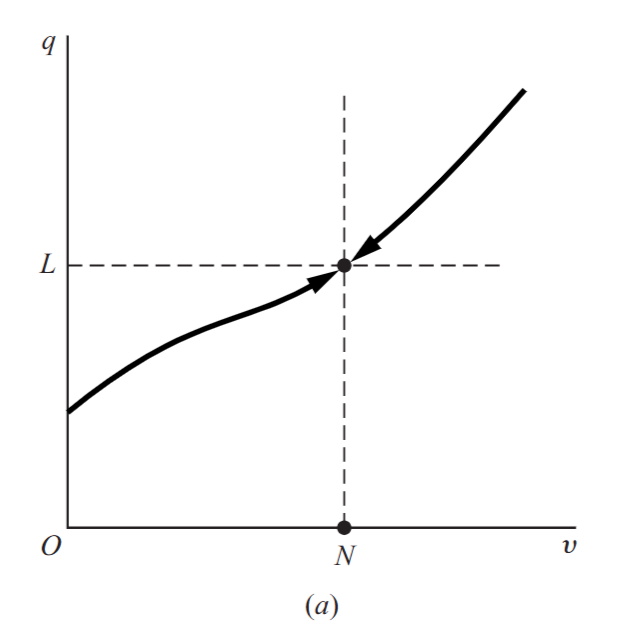
\includegraphics[width=\linewidth,height=0.48\textheight,keepaspectratio]{fig/limits_illustration_a.png}
  \end{minipage}
  \hfill
  \begin{minipage}[t]{0.48\textwidth}
    \centering
    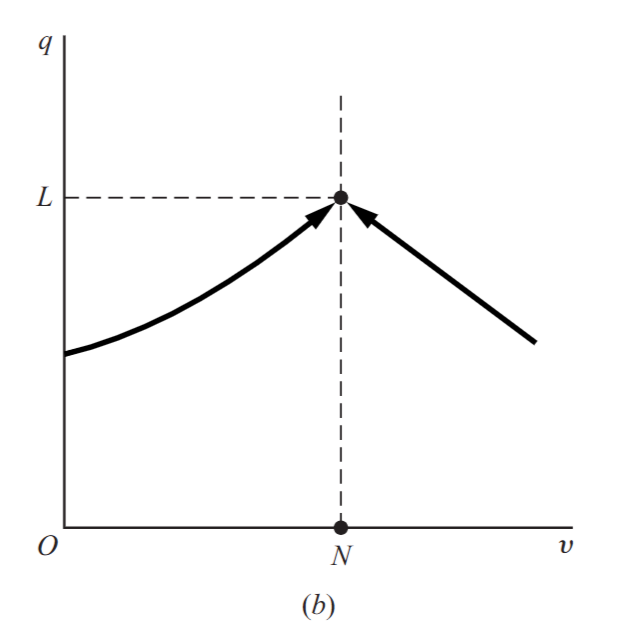
\includegraphics[width=\linewidth,height=0.48\textheight,keepaspectratio]{fig/limits_illustration_b.png}
  \end{minipage}

  % \vspace{0.5em}

  \begin{minipage}[t]{0.48\textwidth}
    \footnotesize
    \textbf{\emph{극한값이 존재}}\\
    \small \textcolor{violet}{$f(\cdot)$}는 'smooth'한 곡선.\\
    좌측에서 \textcolor{blue}{$N$}으로 접근하거나, 우측에서 접근할 시, 모두 극한값이 \textcolor{red}{\emph{L}}로 수렴.
  \end{minipage}
  \hfill
  \begin{minipage}[t]{0.48\textwidth}
    \footnotesize
    \textbf{\emph{극한값이 존재}}\\
    \small \textcolor{violet}{$f(\cdot)$}는 'smooth'하지 \textcolor{magenta}{않는} 곡선.\\
    하지만, 좌측에서 \textcolor{blue}{$N$}으로 접근하거나, 우측에서 접근할 시, 모두 극한값이 \textcolor{red}{\emph{L}}로 수렴.
  \end{minipage}
\end{frame}




\begin{frame}{여러 함수형태에 따른 극한값}
  \begin{minipage}[t]{0.48\textwidth}
    \centering
    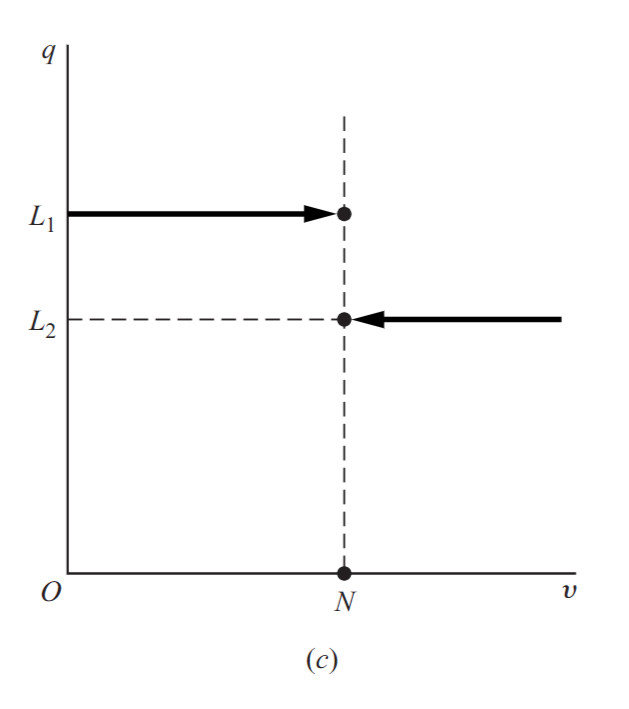
\includegraphics[width=\linewidth,height=0.48\textheight,keepaspectratio]{fig/limits_illustration_c.png}
  \end{minipage}
  \hfill
  \begin{minipage}[t]{0.48\textwidth}
    \centering
    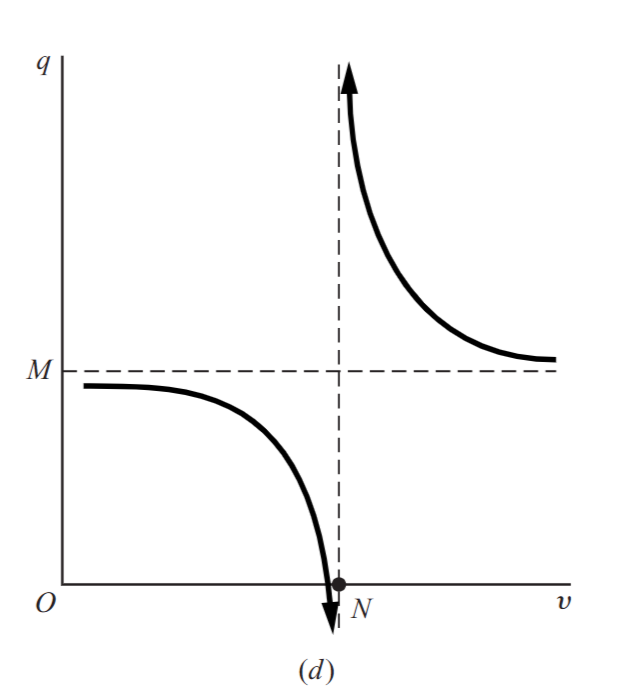
\includegraphics[width=\linewidth,height=0.48\textheight,keepaspectratio]{fig/limits_illustration_d.png}
  \end{minipage}

  % \vspace{0.5em}

  \begin{minipage}[t]{0.48\textwidth}
    \footnotesize
    \textbf{\emph{극한값이 존재하지 \textcolor{magenta}{않음}}}\\
    \scriptsize \textcolor{violet}{$f(\cdot)$}는 'smooth'하지 \textcolor{magenta}{않는} 곡선.\\
    좌측에서 \textcolor{blue}{$N$}으로 접근시 극한값 $L_1$, 우측에서 접근할 시 극한값 $L_2$.\\
    극한값 \textcolor{red}{\emph{L}}이 존재하지 않음.
  \end{minipage}
  \hfill
  \begin{minipage}[t]{0.48\textwidth}
    \footnotesize
    \textbf{\emph{극한값이 존재하지 \textcolor{magenta}{않음}}}\\
    \scriptsize \textcolor{violet}{$f(\cdot)$}는 'smooth'한 곡선.\\
    좌측에서 극한값 $-\infty$, 우측에서 극한값 $\infty$.\\
    따라서 \textcolor{red}{\emph{L}}이 존재하지 않음.
  \end{minipage}
\end{frame}




% \section{지수함수의 극한}
% \begin{frame}{지수함수의 극한 - 일반}
%   \begin{itemize}
%     \item $x \rightarrow a, \, L = f(x)$
%     \item $x \rightarrow \infty, \, L = f(x \mid x=\infty )$
%   \end{itemize}
% \end{frame}





\begin{frame}{함수의 극한: $f(x) = ax$ 의 형태}
  \scriptsize
  \begin{columns}
    % Left column: TikZ plot
    \begin{column}{0.55\textwidth}
      \centering
      
      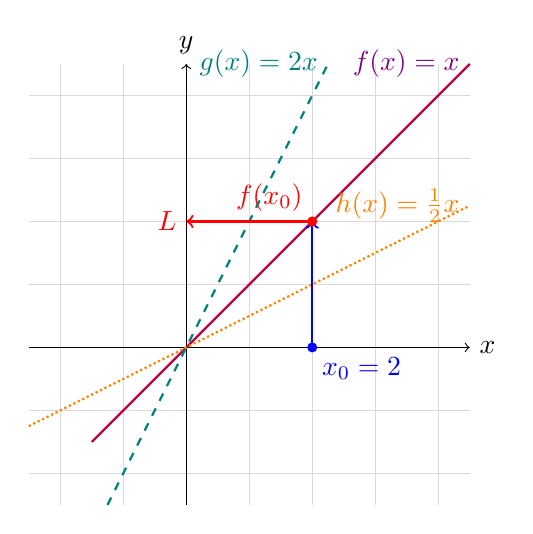
\begin{tikzpicture}[scale=0.8]
        % Grid
        \draw[step=1cm,gray,very thin,opacity=0.3] (-2.5,-2.5) grid (4.5,4.5);
      
        % Axes
        \draw[->] (-2.5,0) -- (4.5,0) node[right] {$x$};
        \draw[->] (0,-2.5) -- (0,4.5) node[above] {$y$};

        % f(x) = x
        \draw[thick,purple] (-1.5,-1.5) -- (4.5,4.5) node[left] {\textcolor{violet}{$f(x) = x$}};
        
        % g(x) = 2x
        \draw[thick,teal,dashed] (-1.25,-2.5) -- (2.25,4.5) node[left] { \textcolor{teal}{$g(x) = 2x$}};

        % h(x) = (1/2)x
        \draw[thick,orange,densely dotted] (-2.5, -1.25) -- (4.5,2.25) node[left] {\textcolor{orange}{$h(x) = \frac{1}{2}x$}};
      
        % Blue dot at a = 2
        \filldraw[blue] (2,0) circle (2pt) node[below right] {$x_0=2$};
        \draw[->,blue,thick] (2,0) -- (2,2);
        
        % Red dot at f(a)
        \filldraw[red] (2,2) circle (2pt) node[above left] {$f(x_0)$};
        \draw[->,red,thick] (2,2) -- (0,2);
        \node[red, left] at (0,2) {$L$};
      \end{tikzpicture}
    \end{column}

    % Right column: description
    \begin{column}{0.45\textwidth}
      \begin{itemize}
        \item $\lim_{x \to 2} \textcolor{violet}{f(x)} = 2$ \\
          $\lim_{x \to 2} \textcolor{teal}{g(x)} = 4$ \\
          $\lim_{x \to 2} \textcolor{orange}{h(x)} = 1/2$
        \item $\lim_{x \to 0} \textcolor{violet}{f(x)} = 0 $ \\
          $\lim_{x \to 0} \textcolor{teal}{g(x)} = 0 $ \\
          $\lim_{x \to 0} \textcolor{orange}{h(x)} = 0 $
        \item $\lim_{x \to \infty} \textcolor{violet}{f(x)} = \infty $ \\
          $\lim_{x \to \infty} \textcolor{teal}{g(x)} = \infty $ \\
          $\lim_{x \to \infty} \textcolor{orange}{h(x)} = \infty $
        \item $\lim_{x \to -\infty} \textcolor{violet}{f(x)} = -\infty $ \\
          $\lim_{x \to -\infty} \textcolor{teal}{g(x)} = -\infty $ \\
          $\lim_{x \to -\infty} \textcolor{orange}{h(x)} = -\infty $
      \end{itemize}
    \end{column}
  \end{columns}
\end{frame}

\begin{frame}{함수의 극한: $f(x) = \dfrac{a}{x}$ 의 형태}
  \scriptsize
  \begin{columns}
    % Left column: TikZ plot
    \begin{column}{0.55\textwidth}
      \centering
      \begin{tikzpicture}[scale=0.65, domain=-4.2:-0.2, samples=100]
        % Grid
        \draw[step=1cm,gray,very thin,opacity=0.3] (-4.5,-4.5) grid (4.5,4.5);

        % Axes
        \draw[->] (-4.5,0) -- (4.5,0) node[right] {$x$};
        \draw[->] (0,-4.5) -- (0,4.5) node[above] {$y$};

        % f(x) = 1/2x → violet
        \draw[thick,violet,densely dotted, domain=-4.2:-0.2] plot (\x, {0.5/\x});
        \draw[thick,violet,densely dotted, domain=0.2:4.2] plot (\x, {0.5/\x}) 
          node[below left] {\textcolor{violet}{$f(x)=\dfrac{1}{2x}$}};

        % g(x) = 1/x → teal
        \draw[thick,teal,dash pattern=on 4pt off 2pt, domain=-4.2:-0.3] plot (\x, {1/\x});
        \draw[thick,teal,dash pattern=on 4pt off 2pt, domain=0.3:4.2] plot (\x, {1/\x}) 
          node[right] {\textcolor{teal}{$g(x)=\dfrac{1}{x}$}};

        % h(x) = 2/x → orange
        \draw[thick,orange,dashed, domain=-4.2:-0.5] plot (\x, {2/\x});
        \draw[thick,orange,dashed, domain=0.5:4.2] plot (\x, {2/\x}) 
          node[above right] {\textcolor{orange}{$h(x)=\dfrac{2}{x}$}};

        % s(x) = 3/x remains purple (unchanged)
        \draw[thick,purple, domain=-4.2:-0.7] plot (\x, {3/\x});
        \draw[thick,purple, domain=0.7:4.2] plot (\x, {3/\x}) 
          node[above left] {\textcolor{purple}{$s(x)=\dfrac{3}{x}$}};

        % Vertical dashed line at x = 0 (asymptote)
        \draw[gray, dashed] (0,-4.5) -- (0,4.5);
      \end{tikzpicture}
    \end{column}

    % Right column: description
    \begin{column}{0.45\textwidth}
      \begin{itemize}
        \item $\lim_{x \to 1} \textcolor{violet}{f(x)} = \frac{1}{2}$ \\
              $\lim_{x \to 1} \textcolor{teal}{g(x)} = 1$ \\
              $\lim_{x \to 1} \textcolor{orange}{h(x)} = 2$
        \item $\lim_{x \to 0^+} \textcolor{violet}{f(x)} = \infty $ \\
              $\lim_{x \to 0^+} \textcolor{teal}{g(x)} = \infty $ \\
              $\lim_{x \to 0^+} \textcolor{orange}{h(x)} = \infty $
        \item $\lim_{x \to 0^-} \textcolor{violet}{f(x)} = -\infty $ \\
              $\lim_{x \to 0^-} \textcolor{teal}{g(x)} = -\infty $ \\
              $\lim_{x \to 0^-} \textcolor{orange}{h(x)} = -\infty $
        \item $\lim_{x \to \infty} \textcolor{violet}{f(x)} = 0 $ \\
              $\lim_{x \to \infty} \textcolor{teal}{g(x)} = 0 $ \\
              $\lim_{x \to \infty} \textcolor{orange}{h(x)} = 0 $
        \item $\lim_{x \to -\infty} \textcolor{violet}{f(x)} = 0^- $ \\
              $\lim_{x \to -\infty} \textcolor{teal}{g(x)} = 0^- $ \\
              $\lim_{x \to -\infty} \textcolor{orange}{h(x)} = 0^- $
        % \item 모든 함수는 $\displaystyle f(x)=\frac{a}{x}$ 꼴이며 $x \ne 0$에서 정의됨.
        % \item $x \to \infty$일 때 $\displaystyle f(x) \to 0$
        % \item $x \to 0^+$ 또는 $x \to 0^-$일 때 수직선 방향에 따라 극한은 $\pm \infty$
        % \item $\displaystyle \lim_{x \to \infty} \frac{a}{x} = 0$ \\
        %       $\displaystyle \lim_{x \to 0^+} \frac{a}{x} = \infty$ (if \( a > 0 \)) \\
        %       $\displaystyle \lim_{x \to 0^-} \frac{a}{x} = -\infty$
        % \item 계수 \( a \)가 커질수록 그래프가 더 가파르게 생김
      \end{itemize}
      % \vspace{0.3em}
      % \textcolor{gray}{\scriptsize 수직 점근선: $x=0$, 수평 점근선: $y=0$}
    \end{column}
  \end{columns}
\end{frame}





\begin{frame}{함수의 극한: $f(x) = x^a$ 의 형태}
  \scriptsize
  \begin{columns}
    % Left column: TikZ plot
    \begin{column}{0.55\textwidth}
      \centering
      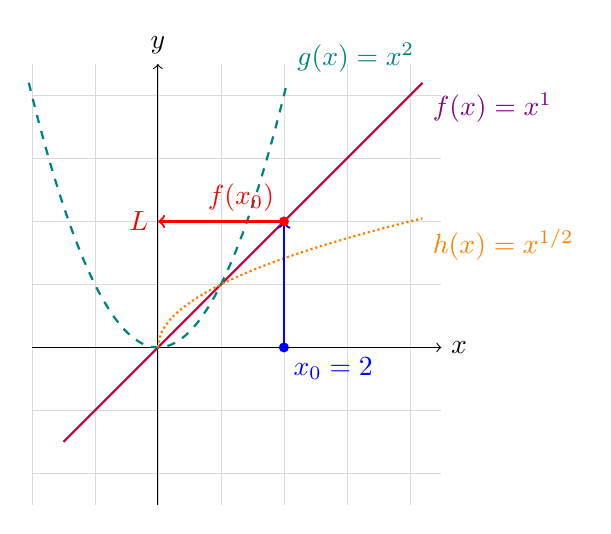
\begin{tikzpicture}[scale=0.8, domain=-1.5:4.2, samples=100]
        % Grid
        \draw[step=1cm,gray,very thin,opacity=0.3] (-2,-2.5) grid (4.5,4.5);
        
        % Axes
        \draw[->] (-2,0) -- (4.5,0) node[right] {$x$};
        \draw[->] (0,-2.5) -- (0,4.5) node[above] {$y$};

        % f(x) = x^1
        \draw[thick,purple] plot (\x, {\x}) node[below right] {\textcolor{violet}{$f(x)=x^1$}};

        % g(x) = x^2 with codomain suppressed to y <= 4.2
        \draw[thick,teal,dashed, domain=-2.05:2.05] plot (\x, {\x*\x}) node[above right] {\textcolor{teal}{$g(x)=x^2$}};

        % h(x) = sqrt(x)
        \draw[thick,orange,densely dotted, domain=0:4.2] plot (\x, {sqrt(\x)}) node[below right] {\textcolor{orange}{$h(x)=x^{1/2}$}};
        
        % Blue vertical line at x = 2
        \filldraw[blue] (2,0) circle (2pt) node[below right] {$x_0=2$};
        \draw[->,blue,thick] (2,0) -- (2,2);

        % Red dot at f(2) = 2
        \filldraw[red] (2,2) circle (2pt) node[above left] {$f(x_0)$};
        \draw[->,red,thick] (2,2) -- (0,2);
        \node[red, left] at (0,2) {$L$};
      \end{tikzpicture}
    \end{column}

    % Right column: description
    \begin{column}{0.45\textwidth}
      \begin{itemize}
        \item $\lim_{x \to 2} \textcolor{violet}{f(x)} = 2$ \\
          $\lim_{x \to 2} \textcolor{teal}{g(x)} = 4$ \\
          $\lim_{x \to 2} \textcolor{orange}{h(x)} = \sqrt{2}$
        \item $\lim_{x \to 0} \textcolor{violet}{f(x)} = DNE$\\
          $\lim_{x \to 0} \textcolor{teal}{g(x)} = 0$\\
          $\lim_{x \to 0} \textcolor{orange}{h(x)} = 0$
        \item $\lim_{x \to \infty} \textcolor{violet}{f(x)} = \infty $ \\
          $\lim_{x \to \infty} \textcolor{teal}{g(x)} = \infty $ \\
          $\lim_{x \to \infty} \textcolor{orange}{h(x)} = \infty $
        \item $\lim_{x \to -\infty} \textcolor{violet}{f(x)} = -\infty $ \\
          $\lim_{x \to -\infty} \textcolor{teal}{g(x)} = \infty $ \\
          $\lim_{x \to -\infty} \textcolor{orange}{h(x)} = DNE $
        \item $\lim_{x \to 0^+} \textcolor{violet}{f(x)} = 0$ \\
          $\lim_{x \to 0^+} \textcolor{teal}{g(x)} = 0$ \\
          $\lim_{x \to 0^+} \textcolor{orange}{h(x)} = 0$ 
      \end{itemize}
      % \vspace{0.3em}
      % \textcolor{gray}{\scriptsize($x > 0$ 영역에서 정의된 함수들 비교 — 특히 $x^{1/2}$는 $x < 0$에서는 정의되지 않음.)}
    \end{column}
  \end{columns}
\end{frame}




\begin{frame}{함수의 극한: $f(x) = a^x$ 의 형태}
  \scriptsize
  \begin{columns}
    % Left column: TikZ plot
    \begin{column}{0.55\textwidth}
      \centering
      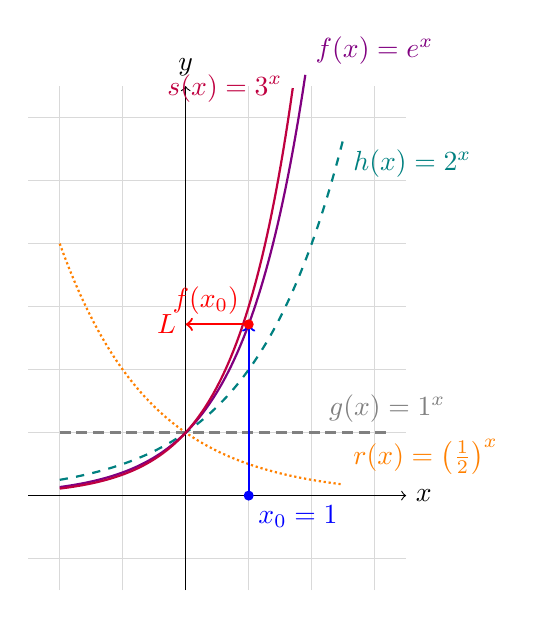
\begin{tikzpicture}[scale=0.8, domain=-2:2.5, samples=100]
        % Grid
        \draw[step=1cm,gray,very thin,opacity=0.3] (-2.5,-1.5) grid (3.5,6.5);
        
        % Axes
        \draw[->] (-2.5,0) -- (3.5,0) node[right] {$x$};
        \draw[->] (0,-1.5) -- (0,6.5) node[above] {$y$};

        % r(x) = (1/2)^x
        \draw[thick,orange,densely dotted] plot (\x, {pow(0.5,\x)}) node[above right] {\textcolor{orange}{$r(x)=\left(\frac{1}{2}\right)^x$}};

        % g(x) = 1^x (constant 1)
        \draw[thick,gray,dash pattern=on 4pt off 2pt] (-2,1) -- (3.2,1) node[above] {\textcolor{gray}{$g(x)=1^x$}};

        % h(x) = 2^x
        \draw[thick,teal,dashed] plot (\x, {pow(2,\x)}) node[below right] {\textcolor{teal}{$h(x)=2^x$}};

        % f(x) = e^x
        \draw[thick,violet, domain=-2:1.9] plot (\x, {exp(\x)}) node[above right] {\textcolor{violet}{$f(x)=e^x$}};

        % s(x) = 3^x
        \draw[thick,purple, domain=-2:1.7] plot (\x, {pow(3,\x)}) node[left] {\textcolor{purple}{$s(x)=3^x$}};

        % Reference vertical line at x = 1
        \filldraw[blue] (1,0) circle (2pt) node[below right] {$x_0=1$};
        \draw[->,blue,thick] (1,0) -- (1,{exp(1)});
        \filldraw[red] (1,{exp(1)}) circle (2pt) node[above left] {$f(x_0)$};
        \draw[->,red,thick] (1,{exp(1)}) -- (0,{exp(1)});
        \node[red,left] at (0,{exp(1)}) {$L$};
      \end{tikzpicture}
    \end{column}

    % Right column: description
    \begin{column}{0.45\textwidth}
      % \begin{itemize}
      %   \item $\textcolor{orange}{\left(\frac{1}{2}\right)^x}$: 감소 함수, $x \to \infty$일 때 0에 수렴
      %   \item $\textcolor{gray}{1^x}$: 항상 1 (상수함수)
      %   \item $\textcolor{teal}{2^x}$: 전형적인 증가 함수
      %   \item $\textcolor{blue}{e^x}$: 미분 가능하고 자연로그의 역함수
      %   \item $\textcolor{violet}{3^x}$: 가장 빠르게 증가
      % \end{itemize}
      % \vspace{0.5em}
      \begin{itemize}
        \item $\lim_{x \to 1} \textcolor{violet}{f(x)} = e $ \\
          $\lim_{x \to 1} \textcolor{teal}{h(x)} = 2 $ \\
          $\lim_{x \to 1} \textcolor{orange}{r(x)} = 1/2 $
        \item $\lim_{x \to \infty} a^x = 
          \begin{cases}
            0 & \text{if } 0 < a < 1 \\
            1 & \text{if } a = 1 \\
            \infty & \text{if } a > 1
          \end{cases}$
        \item $\lim_{x \to -\infty} a^x = 
          \begin{cases}
            \infty & \text{if } 0 < a < 1 \\
            1 & \text{if } a = 1 \\
            0 & \text{if } a > 1
          \end{cases}$
      % \item $ \lim_{x \rightarrow x_0} \textcolor{blue}{e^x} = e^{x_0}$
      \end{itemize}
    \end{column}
  \end{columns}
\end{frame}





\begin{frame}{함수의 극한: $f(x) = \log_a x$ 의 형태}
  \scriptsize
  \begin{columns}
    % Left column: TikZ plot
    \begin{column}{0.55\textwidth}
      \centering
      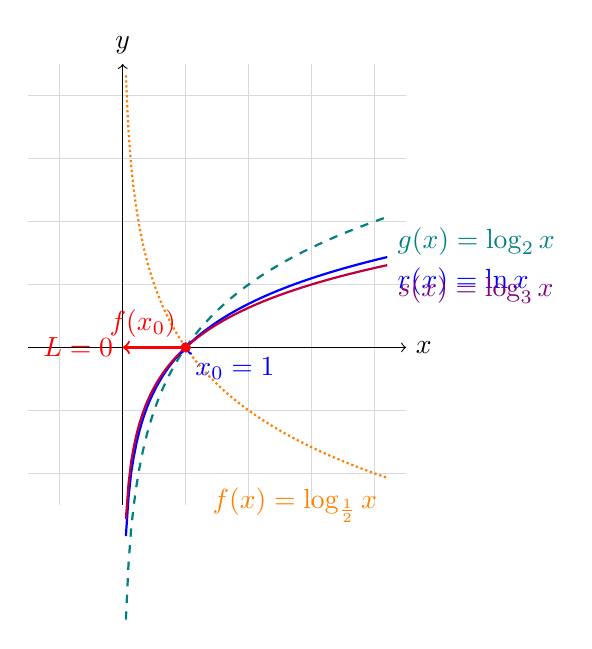
\begin{tikzpicture}[scale=0.8, domain=0.05:4.2, samples=100]
        % Grid
        \draw[step=1cm,gray,very thin,opacity=0.3] (-1.5,-2.5) grid (4.5,4.5);
        
        % Axes
        \draw[->] (-1.5,0) -- (4.5,0) node[right] {$x$};
        \draw[->] (0,-2.5) -- (0,4.5) node[above] {$y$};

        % f(x) = log_{1/2}(x)
        \draw[thick,orange,densely dotted] plot (\x, {ln(\x)/ln(0.5)}) node[below left] {\textcolor{orange}{$f(x)=\log_{\frac{1}{2}} x$}};

        % g(x) = log_1(x) -- undefined: skip plotting

        % h(x) = log_2(x)
        \draw[thick,teal,dashed] plot (\x, {ln(\x)/ln(2)}) node[below right] {\textcolor{teal}{$g(x)=\log_{2} x$}};

        % r(x) = ln(x)
        \draw[thick,blue] plot (\x, {ln(\x)}) node[below right] {\textcolor{blue}{$r(x)=\ln x$}};

        % s(x) = log_3(x)
        \draw[thick,purple] plot (\x, {ln(\x)/ln(3)}) node[below right] {\textcolor{violet}{$s(x)=\log_{3} x$}};

        % Vertical reference line at x = 1
        \filldraw[blue] (1,0) circle (2pt) node[below right] {$x_0=1$};
        \draw[->,blue,thick] (1,0) -- (1,{ln(1)});
        \filldraw[red] (1,0) circle (2pt) node[above left] {$f(x_0)$};
        \draw[->,red,thick] (1,0) -- (0,0);
        \node[red,left] at (0,0) {$L=0$};
      \end{tikzpicture}
    \end{column}

    % Right column: description
    \begin{column}{0.45\textwidth}
      \begin{itemize}
        \item $x > 0$일 때 정의됨. $x \to 0^+$에서 $\log_a x \to -\infty$
        \item $\textcolor{orange}{\log_{\frac{1}{2}} x}$: 감소 함수
        \item $\textcolor{teal}{\log_2 x}$, $\textcolor{violet}{\log_3 x}$, $\textcolor{blue}{\ln x}$: 증가 함수
        \item $\log_1 x$는 정의되지 않음 (base 1 불가능)
        \item $\lim_{x \to 1} \log_a x = 0$ \quad (모든 $a > 0$, $a \neq 1$)
        \item $\lim_{x \to \infty} \log_a x = 
          \begin{cases}
            -\infty & \text{if } 0 < a < 1 \\
            \infty & \text{if } a > 1
          \end{cases}$
      \end{itemize}
    \end{column}
  \end{columns}
\end{frame}








\section{절대값함수의 극한}
\begin{frame}{Visualizing $f(x) = |x|$ at $a = 2$}
  \centering
  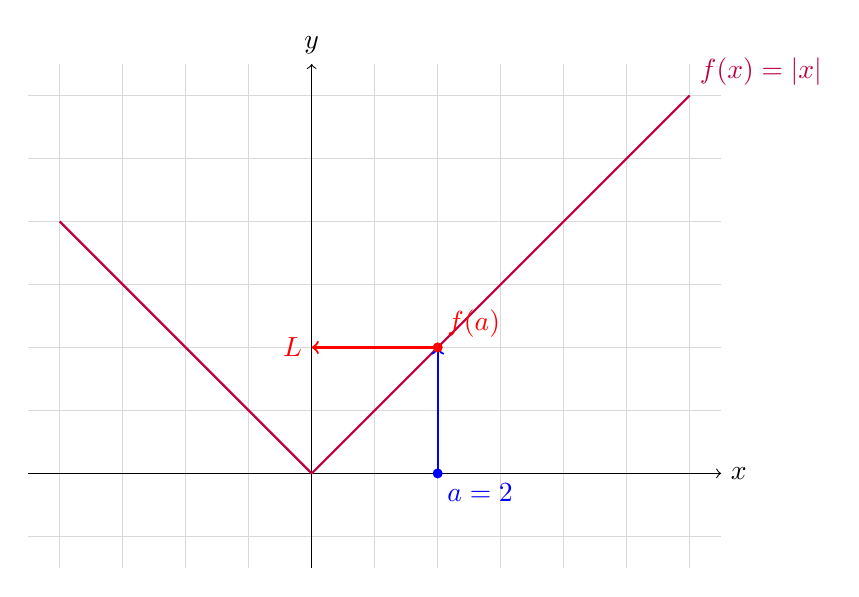
\begin{tikzpicture}[scale=0.8]
    % Grid
    \draw[step=1cm,gray,very thin,opacity=0.3] (-4.5,-1.5) grid (6.5,6.5);
  
    % Axes
    \draw[->] (-4.5,0) -- (6.5,0) node[right] {$x$};
    \draw[->] (0,-1.5) -- (0,6.5) node[above] {$y$};
  
    % Function f(x) = |x|
    \draw[domain=-4:0,smooth,variable=\x,thick,purple] 
      plot ({\x},{-1*\x});
    \draw[domain=0:6,smooth,variable=\x,thick,purple] 
      plot ({\x},{\x}) node[anchor=south west] {\textcolor{purple}{$f(x) = |x|$}};
  
    % Blue dot at a = 2
    \filldraw[blue] (2,0) circle (2pt) node[below right] {$a=2$};
    \draw[->,blue,thick] (2,0) -- (2,2);
  
    % Red dot at f(a)
    \filldraw[red] (2,2) circle (2pt) node[above right] {$f(a)$};
    \draw[->,red,thick] (2,2) -- (0,2);
    \node[red, left] at (0,2) {$L$};
  \end{tikzpicture}
\end{frame}


\section{계단함수의 극한}
% \section{지수함수의 극한}
\begin{frame}{Visualizing $f(x) = \lfloor x \rfloor$ at $a = 2$}
  \centering
  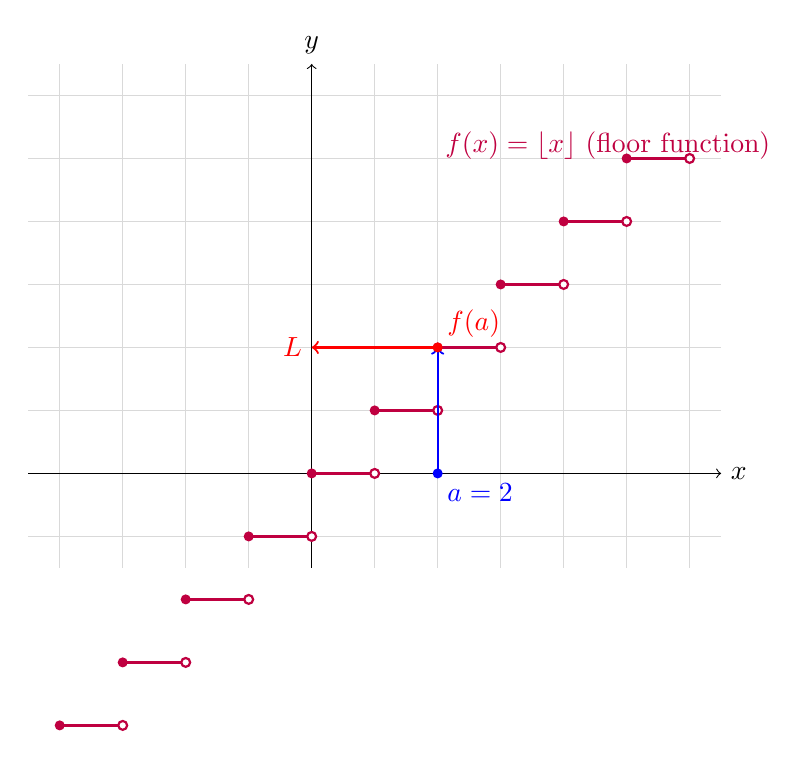
\begin{tikzpicture}[scale=0.8]
    % Grid
    \draw[step=1cm,gray,very thin,opacity=0.3] (-4.5,-1.5) grid (6.5,6.5);
  
    % Axes
    \draw[->] (-4.5,0) -- (6.5,0) node[right] {$x$};
    \draw[->] (0,-1.5) -- (0,6.5) node[above] {$y$};
  
    % Floor function
    \foreach \x in {-4,...,5} {
      \draw[thick, purple] (\x,\x) -- (\x+1,\x);
      \draw[thick, purple, fill=white] (\x+1,\x) circle (2pt); % open circle
      \filldraw[purple] (\x,\x) circle (2pt); % closed circle
    }
    \node[purple] at (4.7,5.2) {$f(x) = \lfloor x \rfloor$ (floor function)};
  
    % Blue dot at a = 2
    \filldraw[blue] (2,0) circle (2pt) node[below right] {$a=2$};
    \draw[->,blue,thick] (2,0) -- (2,2);
  
    % Red dot at f(a) = floor(2) = 2
    \filldraw[red] (2,2) circle (2pt) node[above right] {$f(a)$};
    \draw[->,red,thick] (2,2) -- (0,2);
    \node[red, left] at (0,2) {$L$};
  \end{tikzpicture}
\end{frame}


\section{극한의 성질}
\begin{frame}{극한의 성질}
  함수 \( y = f(x) \) 에 대해 (단, \( a \) 와 \( b \) 는 상수),
  \begin{itemize}
    \item \textbf{정리 I}  \\
    \( y = ax + b \) 일 때,  
    \( \lim_{x \to c} y = ac + b \)  
    
    \item \textbf{정리 II}  \\
    \( y = f(x) = b \) (상수 함수) 일 때,  
    \( \lim_{x \to c} y = b \)  
    % 즉, 상수 함수의 극한은 해당 상수입니다.  
    % 이는 \( a = 0 \) 인 정리 I의 특수한 경우입니다.

    \item \textbf{정리 III}  \\
    \( y = x \) 일 때, \( \lim_{x \to c} y = c \),   \\
    \( y = x^k \) 일 때, \( \lim_{x \to c} y = c^k \)  
  \end{itemize}
  % 이 세 정리에서는 \( x = c \) 를 직접 대입해 극한값을 구할 수 있지만,  이는 특수한 경우일 뿐이며, 
  \emph{*일반적으로는 “\( x \to c \)” 는 “\( x = c \)” 와 같지 않음 (대입시 다른 값).}

  % \vspace{0.5cm}

  \begin{itemize}
    \item \textbf{예시 1:} \( y = 5x + 7 \)  
    \[
      \lim_{x \to 2} y = 5(2) + 7 = 17,\quad
      \lim_{x \to 0} y = 5(0) + 7 = 7
    \]

    \item \textbf{예시 2:} \( y = x^3 \)  
    \[
      \lim_{x \to 2} y = (2)^3 = 8
    \]
  \end{itemize}
\end{frame}



\begin{frame}{극한의 성질 (두 함수의 조합)}
  두 개의 함수 \( y_1 = f(x) \), \( y_2 = g(x) \) 가 \( x \) 에 대해 주어지고, 다음과 같은 유한한 실수의 극한값을 가질 때:
  \[
    \lim_{x \to c} y_1 = L_1, \quad \lim_{x \to c} y_2 = L_2
  \]
  % 여기서 \( L_1 \)과 \( L_2 \)는 유한한 실수라고 할 때, 다음 정리들이 적용됩니다.
  
  % \vspace{0.4cm}

  \begin{itemize}
    \item \textbf{정리 IV (합/차의 극한)}
    \[
      \lim_{x \to c} (y_1 \pm y_2) = L_1 \pm L_2
    \]
    % 두 함수의 합(또는 차)의 극한은, 각 함수의 극한의 합(또는 차)과 같습니다.

    % \vspace{0.2cm}
    % 예: 
    % \[
    %   \lim_{x \to c} 2y_1 = \lim_{x \to c} (y_1 + y_1) = L_1 + L_1 = 2L_1
    % \]
    % 이는 앞서 배운 \textbf{정리 I}과 일치합니다.
    
    % \vspace{0.5cm}

    \item \textbf{정리 V (곱의 극한)}
    \[
      \lim_{x \to c} (y_1 \cdot y_2) = L_1 \cdot L_2
    \]
    % 두 함수의 곱의 극한은, 각 극한값의 곱과 같습니다.

    % \vspace{0.2cm}
    % 특히, 함수의 제곱에 적용하면:
    % \[
    %   \lim_{x \to c} (y_1)^2 = L_1^2
    % \]
    % 이는 \textbf{정리 III}와 일치합니다.

    % \vspace{0.5cm}

    \item \textbf{정리 VI (나눗셈의 극한)}  
    단, \( L_2 \ne 0 \) 이어야 함
    \[
      \lim_{x \to c} \frac{y_1}{y_2} = \frac{L_1}{L_2}
    \]
    % 두 함수의 비의 극한은, 각 극한값의 비와 같습니다.  
    % 단, 분모의 극한 \( L_2 \) 가 0이 아니어야 의미가 정의됩니다.
  \end{itemize}
\end{frame}

\begin{frame}{다항식 함수의 극한}
  주어진 극한의 성질을 활용하면, 모든 다항식 함수의 극한을 쉽게 구할 수 있습니다.

  \vspace{0.3cm}
  일반적인 다항식 함수:
  \[
    y = f(x) = a_0 + a_1x + a_2x^2 + \cdots + a_nx^n
  \]

  \( x \to c \) 일 때, 각 항의 극한은 다음과 같습니다:
  \[
    \lim_{x \to c} a_0 = a_0, \quad
    \lim_{x \to c} a_1x = a_1c, \quad
    \lim_{x \to c} a_2x^2 = a_2c^2, \quad \cdots
  \]

  \vspace{0.3cm}
  따라서 전체 다항식의 극한은 다음과 같이 계산됩니다:
  \[
    \lim_{x \to c} f(x) = a_0 + a_1c + a_2c^2 + \cdots + a_nc^n
  \]

  % \vspace{0.3cm}
  % 즉, 극한값은 \( x = c \) 를 대입한 함수값 \( f(c) \) 와 같습니다.  
  % 이 사실은 다항식 함수의 **연속성** 개념을 이해하는 데 중요합니다.
\end{frame}


\begin{frame}{예제 1: 다항식 함수의 극한}
  함수 \( y = f(x) = x^2 - 9x + 7 \) 의 극한을 구하시오:
  \begin{itemize}
    \item[(a)] \( \lim_{x \to 0} f(x) \uncover<2->{ = 0^2 - 9(0) + 7 = 7} \)
    \vspace{0.3cm}
    \item[(b)] \( \lim_{x \to 3} f(x) \uncover<2->{ = 3^2 - 9(3) + 7 = 9 - 27 + 7 = -11} \)
    \vspace{0.3cm}
    \item[(c)] \( \lim_{x \to -1} f(x) \uncover<2->{ = (-1)^2 - 9(-1) + 7 = 1 + 9 + 7 = 17} \)
  \end{itemize}
\end{frame}

\begin{frame}{예제 2: 곱 형태의 극한}
함수 \( y = f(x) = (x + 2)(x - 3) \) 의 극한을 구하시오:
\begin{itemize}
  \item[(a)] \( \lim_{x \to -1} f(x) \uncover<2->{ = (-1 + 2)(-1 - 3) = (1)(-4) = -4} \)
  \vspace{0.3cm}
  \item[(b)] \( \lim_{x \to 0} f(x) \uncover<2->{ = (0 + 2)(0 - 3) = (2)(-3) = -6} \)
  \vspace{0.3cm}
  \item[(c)] \( \lim_{x \to 5} f(x) \uncover<2->{ = (5 + 2)(5 - 3) = (7)(2) = 14} \)
\end{itemize}
\end{frame}

\begin{frame}{예제 3: 분수 함수의 극한}
함수 \( y = f(x) = \frac{3x + 5}{x + 2} \) 의 극한을 구하시오:
\begin{itemize}
  \item[(a)] \( \lim_{x \to 0} f(x) \uncover<2->{ = \frac{3(0) + 5}{0 + 2} = \frac{5}{2}} \)
  \vspace{0.3cm}
  \item[(b)] \( \lim_{x \to 5} f(x) \uncover<2->{ = \frac{3(5) + 5}{5 + 2} = \frac{20}{7}} \)
  \vspace{0.3cm}
  \item[(c)] \( \lim_{x \to -1} f(x) \uncover<2->{ = \frac{3(-1) + 5}{-1 + 2} = \frac{-3 + 5}{1} = 2} \)
\end{itemize}
\end{frame}












\section{극한 찾기}
\begin{frame}{극한 형태에서 값 찾기}
  \begin{columns}
    \begin{column}{0.5\textwidth}
      \begin{itemize}
        \item \( \lim \frac{c}{c} = 1 \) \\
              \textcolor{gray}{(같은 상수의 나눗셈)}
        \item \( \lim \frac{c}{\infty} = 0 \) \\
              \textcolor{gray}{(큰 분모 → 값이 작아짐)}
        \item \( \lim \frac{c}{0^+} = +\infty \) \\
              \textcolor{gray}{(작은 양수로 나누면 발산)}
        \item \( \lim \frac{0}{\infty} = 0 \) \\
              \textcolor{gray}{(0이 아무리 큰 수로 나눠져도 0)}
        \item \( \lim \frac{\infty}{0^+} = +\infty \) \\
              \textcolor{gray}{(큰 수를 작은 수로 나누면 발산)}
      \end{itemize}
    \end{column}
    \begin{column}{0.5\textwidth}
      \begin{itemize}
        \item \( \lim \frac{\infty}{\infty} \): \textcolor{red}{불확정형} \\
              \textcolor{gray}{(함수 전개 필요, 예: 다항식의 차수 비교)}
        \item \( \lim \frac{0}{0} \): \textcolor{red}{불확정형} \\
              \textcolor{gray}{(인수분해, 유리화, L'Hôpital 등 필요)}
      \end{itemize}
      \vspace{1em}
      \textbf{※ 불확정형은 직접 계산이나 정리가 필요합니다.}
    \end{column}
  \end{columns}
\end{frame}



\begin{frame}{기본 극한 예시}
  \begin{itemize}
    \item \( \lim_{x \to \infty} \frac{5}{x} = 0 \)
    \item \( \lim_{x \to 0^+} \frac{1}{x} = \infty \)
    \item \( \lim_{x \to 0} \frac{x^2}{x} = 0 \)
    \item \( \lim_{x \to \infty} \frac{x}{x^2} = 0 \)
    \item \( \lim_{x \to \infty} \frac{x^2 + 1}{x^2 - 3} = 1 \)
  \end{itemize}
\end{frame}



\begin{frame}{$ \infty / \infty $ 형태}
  \textbf{형태}: \( \lim_{x \to \infty} \frac{f(x)}{g(x)} = \frac{\infty}{\infty} \) 는 \textcolor{red}{불확정형}

  \vspace{0.5em}
  \textbf{전개 방법:} 최고차항 비교, 인수 정리 또는 L'Hôpital 적용

  \vspace{1em}
  \textbf{예시:}
  \[
    \lim_{x \to \infty} \frac{3x^2 + 2x}{5x^2 - x} = \frac{3}{5}
  \]
  \textcolor{gray}{→ 최고차항으로 나누기}

  \[
    \lim_{x \to \infty} \frac{e^x}{x^3} = \infty
  \]
  \textcolor{gray}{→ 지수가 다항보다 빠르게 성장}
\end{frame}



\begin{frame}{$ 0 / 0 $ 형태}
  \textbf{형태}: \( \lim_{x \to c} \frac{f(x)}{g(x)} = \frac{0}{0} \) 는 \textcolor{red}{불확정형}

  \vspace{0.5em}
  \textbf{해결 방법:}
  \begin{itemize}
    \item 인수분해, 유리화, 공통 인자 소거
    \item 혹은 L'Hôpital Rule 적용
  \end{itemize}

  \vspace{1em}
  \textbf{예시:}
  \[
    \lim_{x \to 2} \frac{x^2 - 4}{x - 2} = \lim_{x \to 2} \frac{(x-2)(x+2)}{x-2} = 4
  \]

  \[
    \lim_{x \to 0} \frac{\sin x}{x} = 1
  \]
\end{frame}


\begin{frame}{L'Hôpital's Rule}
  \textbf{정리 조건:}
  \begin{itemize}
    \item \( \lim_{x \to c} \frac{f(x)}{g(x)} = \frac{0}{0} \) 또는 \( \frac{\infty}{\infty} \)
    \item \( f'(x), g'(x) \) 존재하고, \( g'(x) \neq 0 \)
  \end{itemize}

  \vspace{0.5em}
  \textbf{공식:}
  \[
    \lim_{x \to c} \frac{f(x)}{g(x)} = \lim_{x \to c} \frac{f'(x)}{g'(x)}
  \]

  \vspace{1em}
  \textbf{예시:}
  \[
    \lim_{x \to 0} \frac{\sin x}{x} = \lim_{x \to 0} \frac{\cos x}{1} = 1
  \]

  \[
    \lim_{x \to \infty} \frac{\ln x}{x} = \lim_{x \to \infty} \frac{1/x}{1} = 0
  \]
\end{frame}




\begin{frame}{도함수는는 불확정형 $ 0 / 0 $}
  \begin{definition}[도함수]
    실수($\mathbb{R}$)의 어떤 함수 \textcolor{violet}{$f(x)$}가 정의되는 포인트 \textcolor{blue}{\emph{$a$}} 에서 \emph{미분가능(differentiable)} 하고, 정의역이 포인트 \textcolor{blue}{\emph{$a$}} 를 포함한다면, \textcolor{blue}{\emph{$a$}} 에서 \textcolor{red}{미분계수(순간변화율)} \textcolor{red}{\emph{$L$}} 은 \\
    \begin{equation}
      \textcolor{red}{L} = \textcolor{teal}{\lim_{h \to 0} \frac{f(\textcolor{blue}{a}+h)-f(\textcolor{blue}{a})}{h}}
    \end{equation}
  \end{definition}
  \vspace{10pt}
  도함수는 $0/0$의 불확정형태를 가지고 있음. 도함수의 정의를 의용해서 미분계수를 구할때는 인수분해, 유리화, 통 인자 소거 혹은 L'Hôpital Rule 을 적용하여야 함. \\
  이처럼 극한은 미분의 근본을 구성하며, 극한의 성질을 이해하는것이 미분을 이해하는데 중요함. 다시한번 강조하지만, 미분가능성의 조건은 포인트 \textcolor{blue}{\emph{$a$}} 에서 올바른 극한값의 조건을 만족해야 함.
\end{frame}



\section{경제학에서 사용하는 함수와 극한}

\begin{frame}{콥더글라스 생산함수}
  \scriptsize
  \begin{columns}
    % Left column: TikZ plot
    \begin{column}{0.55\textwidth}
      \centering
      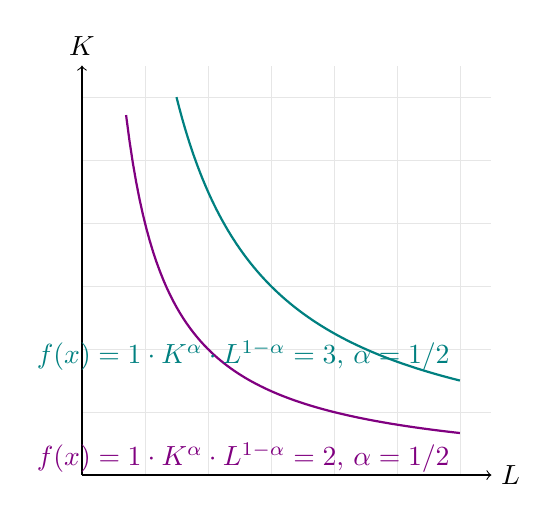
\begin{tikzpicture}[scale=0.8, domain=.5:6, samples=100]
        % Grid
        \draw[step=1cm,gray,very thin,opacity=0.2] (0,0) grid (6.5,6.5);
        
        % Axes
        \draw[->] (0,0) -- (6.5,0) node[right] {$L$};
        \draw[->] (0,0) -- (0,6.5) node[above] {$K$};

        % f(x) = x^1
        % \draw[thick,purple] plot (\x, {\x}) node[below right] {\textcolor{violet}{$f(x)=x^1$}};
        
        % f(x) = 1*K^.5*L^.5 = 4
        \draw[thick,violet, domain=.7:6] plot (\x,{4/(\x)}) node[below left] {\textcolor{violet}{$f(x) = 1 \cdot K^{\alpha} \cdot L^{1-\alpha} = 2, \, \alpha = 1/2$}};

        % g(x) = 1*K^.5*L^.5 = 4
        \draw[thick,teal, domain=1.5:6] plot (\x,{9/(\x)}) node[above left] {\textcolor{teal}{$f(x) = 1 \cdot K^{\alpha} \cdot L^{1-\alpha} = 3, \, \alpha = 1/2$}};

      \end{tikzpicture}
    \end{column}

    % Right column: description
    \begin{column}{0.45\textwidth}
      \textbf{함수형태:} \( f(K, L) = A K^\alpha L^\beta \)

      \begin{itemize}
        \item \( A > 0 \), \( 0 < \alpha, \beta < 1 \)
        \item 생산요소 \( K, L \)이 증가할 때 산출물의 극한 분석
      \end{itemize}
    
      \vspace{0.5em}
      \textbf{예시:}
      \[
        \lim_{K \to \infty} A K^\alpha L^\beta = \infty \quad (\text{고정 } L > 0)
      \]
      \textcolor{gray}{→ 규모의 경제 또는 한계생산체감 여부를 확인}
    
      \[
        \lim_{K \to 0^+} A K^\alpha L^\beta = 0
      \]
      \textcolor{gray}{→ 자본이 없는 경우 산출물도 없음}
      % \vspace{0.3em}
      % \textcolor{gray}{\scriptsize($x > 0$ 영역에서 정의된 함수들 비교 — 특히 $x^{1/2}$는 $x < 0$에서는 정의되지 않음.)}
    \end{column}
  \end{columns}
\end{frame}








\begin{frame}{유리함수 형태의 효용함수}
  \scriptsize
  \begin{columns}
    % Left column: TikZ plot
    \begin{column}{0.55\textwidth}
      \centering
      \begin{tikzpicture}[scale=0.8, domain=.5:6, samples=100]
        % Grid
        \draw[step=1cm,gray,very thin,opacity=0.2] (0,0) grid (6.5,6.5);
        
        % Axes
        \draw[->] (0,0) -- (6.5,0) node[right] {$L$};
        \draw[->] (0,0) -- (0,6.5) node[above] {$K$};

        
        % f(x) = 1/2x → violet
        % \draw[thick,violet,densely dotted, domain=-4.2:-0.2] plot (\x, {0.5/\x});
        \draw[thick,violet,densely dotted, domain=0.2:4.2] plot (\x, {0.5/\x}) 
          node[below left] {\textcolor{violet}{$f(x)=\dfrac{1}{2x}$}};
        
        % % f(x) = 1*K^.5*L^.5 = 4
        % \draw[thick,violet, domain=.7:6] plot (\x,{4/(\x)}) node[below left] {\textcolor{violet}{$f(x) = 1 \cdot K^{\alpha} \cdot L^{1-\alpha} = 2, \, \alpha = 1/2$}};

        % % g(x) = 1*K^.5*L^.5 = 4
        % \draw[thick,teal, domain=1.5:6] plot (\x,{9/(\x)}) node[above left] {\textcolor{teal}{$f(x) = 1 \cdot K^{\alpha} \cdot L^{1-\alpha} = 3, \, \alpha = 1/2$}};

      \end{tikzpicture}
    \end{column}

    % Right column: description
    \begin{column}{0.45\textwidth}
      \textbf{함수형태:} \( U(x) = \frac{a x}{b + x} \)

      \begin{itemize}
        \item 한계효용체감 (Diminishing Marginal Utility) 설명
        \item 상한값(포화효용)에 접근함
      \end{itemize}
    
      \vspace{0.5em}
      \textbf{예시:}
      \[
        \lim_{x \to \infty} \frac{a x}{b + x} = a
      \]
      \textcolor{gray}{→ 효용이 한계값 \( a \)에 수렴}
    
      \[
        \lim_{x \to 0} \frac{a x}{b + x} = 0
      \]
    \end{column}
  \end{columns}
\end{frame}







% % f(x) = 1/2x → violet
% \draw[thick,violet,densely dotted, domain=-4.2:-0.2] plot (\x, {0.5/\x});
% \draw[thick,violet,densely dotted, domain=0.2:4.2] plot (\x, {0.5/\x}) 
%   node[below left] {\textcolor{violet}{$f(x)=\dfrac{1}{2x}$}};


% \begin{frame}{유리함수 - 효용함수}
%   \textbf{함수형태:} \( U(x) = \frac{a x}{b + x} \)

%   \begin{itemize}
%     \item 한계효용체감 (Diminishing Marginal Utility) 설명
%     \item 상한값(포화효용)에 접근함
%   \end{itemize}

%   \vspace{0.5em}
%   \textbf{예시:}
%   \[
%     \lim_{x \to \infty} \frac{a x}{b + x} = a
%   \]
%   \textcolor{gray}{→ 효용이 한계값 \( a \)에 수렴}

%   \[
%     \lim_{x \to 0} \frac{a x}{b + x} = 0
%   \]
% \end{frame}


% \begin{frame}{지수함수 - 효용함수}
%   \textbf{함수형태:} \( U(x) = 1 - e^{-a x} \), \( a > 0 \)

%   \begin{itemize}
%     \item 위험회피적(agent risk-averse) 효용 함수
%     \item 빠르게 증가하지만 수렴 (bounded)
%   \end{itemize}

%   \vspace{0.5em}
%   \textbf{예시:}
%   \[
%     \lim_{x \to \infty} \left(1 - e^{-a x}\right) = 1
%   \]
%   \textcolor{gray}{→ 효용은 상한값 1에 접근}

%   \[
%     \lim_{x \to 0} \left(1 - e^{-a x}\right) = 0
%   \]
% \end{frame}



% \begin{frame}{완전대체제 선형함수}
%   \textbf{함수형태:} \( U(x, y) = a x + b y \)

%   \begin{itemize}
%     \item 소비재 간 완전 대체 관계 (직선 무차별 곡선)
%     \item 극한 분석을 통해 가격비 분석 가능
%   \end{itemize}

%   \textbf{예시:}
%   \[
%     \lim_{x \to \infty} U(x, y) = \infty \quad (\text{고정 } y > 0)
%   \]
%   \textcolor{gray}{→ 특정 소비재에 집중된 효용 증가}
% \end{frame}


% \begin{frame}{완전보완제 레온티예프프함수}
%   \textbf{함수형태:} \( U(x, y) = \min(ax, by) \)

%   \begin{itemize}
%     \item 보완재 간 비율에 따라 효용 결정
%     \item 극한에서 불균형 소비는 효용 제한
%   \end{itemize}

%   \vspace{0.5em}
%   \textbf{예시:}
%   \[
%     \lim_{x \to \infty} \min(ax, by) = by \quad (\text{고정 } y)
%   \]
%   \[
%     \lim_{x \to 0^+} \min(ax, by) = 0
%   \]
%   \textcolor{gray}{→ 한 쪽이 없으면 전체 효용도 없음}
% \end{frame}









% \section{생산함수: 콥더글라스}

% \section{효용함수: 유리함수}

% \section{완전대체제: 선형함수}

% \section{완전보완제: 레온티예프}



\end{document}

